% we need to provide something to fool the setting of \bibsep
\newdimen\bibsep
%%%

\documentclass[review,11pt,nonatbib]{elsarticle}
\usepackage{setspace}
\usepackage{lineno}
\usepackage{color}
%\usepackage{hyperref}
\usepackage[top=2.54cm , bottom=2.54cm, left=2.54cm, right=2.54cm]{geometry}
\usepackage{amsmath}
\usepackage{amssymb}
\usepackage{graphicx}
\usepackage{booktabs}
\usepackage{subfigure}
\usepackage{color}
\usepackage{multirow}
\usepackage{mathrsfs}
\usepackage{bm}
\usepackage{mathptm}

\usepackage[style=apa6,natbib=true]{biblatex}

\addbibresource{mybibfile.bib}

\journal{}
%%
%To fix the line number

%%%%%%%%%%%%%%%%%%%%%%%
%% Elsevier bibliography styles
%%%%%%%%%%%%%%%%%%%%%%%
%% To change the style, put a % in front of the second line of the current style and
%% remove the % from the second line of the style you would like to use.
%%%%%%%%%%%%%%%%%%%%%%%

%% Numbered

%%%%%%%%%%%%%%%%%%%%%%%

\begin{document}

\begin{frontmatter}

\title{An explicit approach for modeling the performance of transportation networks immediately after an earthquake}
\author[add1,add2]{Kairui Feng}
\author[add3]{Cao Wang}
\author[add1]{Quanwang Li\corref{ca}}

\cortext[ca]{Corresponding author. Email addresses: li\_quanwang@tsinghua.edu.cn (Q.Li).}
\address[add1]{Department of Civil Engineering, Tsinghua University, Beijing 100084, China}
\address[add2]{Department of Civil and Environmental Engineering, Princeton University, Princeton, NJ 08540, USA}
\address[add3]{School of Civil, Mining and Environmental Engineering, University of Wollongong, Wollongong, NSW 2522, Australia}

\begin{abstract}
  Surface transportation systems play a vital role in supporting a region's functionalities. They are expected to remain operational before and even after a hazardous event (e.g., an earthquake). The importance is evident to estimate the post-disaster performance of traffic systems under a probability-based framework, considering the uncertainties arising from both the hazards and the transportation infrastructure fragilities. This paper proposes an explicit approach for evaluating the performance of transportation systems immediately after an earthquake event. The method estimates the spatial distribution of vehicles in the traffic network in a closed form, and thus is relatively efficient compared with traditional methods (e.g., an agent-based method). The applicability of the proposed approach is demonstrated through an application to the post-earthquake performance assessment of the traffic network in Tangshan City, China, a city that suffered catastrophically from the 1976 Tangshan Earthquake. Analytical results show that the proposed method can well reflect both the temporal and the spatial variations of the traffic flow, and thus offers a rational support for predicting the post-earthquake traffic scenarios and for optimizing strategies to improve the transportation capability under emergent conditions.
\end{abstract}

\begin{keyword}
transportation network \sep real-time modeling \sep earthquake \sep explicit approach \sep post-disaster response \sep Emergency Management \sep Hospital System
\end{keyword}

\end{frontmatter}

%\linenumbers
\section{Introduction}
Urban transportation systems are a major part of public civil infrastructure, which play an important role in the economy development of a city and the well-beings of its residents. Under emergency conditions, e.g., immediately after an earthquake, transportation systems are also in urgent need for the movement of search/rescue personnel and medical teams, and for transferring injured people to healthcare facilities. In this respect, it is critically important that the transportation systems remain operational following a disaster event so that the movement of emergency response vehicles will not be impeded by severe congestion and excessive delay.
\par To evaluate the performance of transportation systems following an earthquake event, it is essential to understand and model the traffic flow in an emergency situation \citep{brodsky1990emergency,jacques2014resilience,miller2016coupling}. The seismic damages to bridges and other components in the transportation network are spatially distributed over a large area, uncertain and spatially correlated \citep{Han2012Probabilistic}. To represent the spatial variation of seismic damage to transportation systems and investigate its impact on the performance of transportation network, a probabilistic framework for post-earthquake modeling and risk assessment is needed, which starts from the realization of spatially-varied random variables (e.g., ground shaking intensity and damage state of transportation components), and then evaluates the performance of the transportation network for each event realization \citep{Grossi2005Catastrophe,Han2012Probabilistic,Miller2015Estimating}. 

The modeling of traffic flow immediately following an earthquake is sophisticated because many drivers may change their routes and additional traffic demands are induced by the transportation of emergency response teams following the earthquake \citep{ahn2014study}. In that case, the dynamic traffic assignment (DTA) has to be used to predict the traffic pattern and congestion formation in networks \citep{Szeto2011A,Tanimoto2015}. However, the DTA of a realistic urban transportation system is computationally expensive, and the assumption that the drivers come to an equilibrium spontaneously and immediately in the network is unsuitable for immediate post-earthquake traffic flow modeling, because drivers lack the information on traffic congestion to select appropriate alternative routes or may be experiencing panic \citep{pel2011modelling}. Therefore, the fully probabilistic performance assessment presents a challenge to the post-earthquake modeling of transportation systems.
\par Due to the aforementioned challenges, one of the frequently-used methods is to consider a simplified network and a static network flow for seismic risk assessment \citep{Duenas2007Seismic,Miller2015Estimating}, which, however, cannot capture the abnormal characteristics of traffic condition induced by the damaged traffic capacity and the irrational behavior of drivers following an earthquake. Another approach is to simply focus on a single scenario event instead of the fully probabilistic performance assessment  \citep{freckleton2012evaluation,chang2012post,feng2017post}, which cannot take into account the uncertainties associated with the hazards as well as the damage states of the infrastructure components. Especially, agent-based methods, such as ref. \citet{feng2017post}, which store and simulate the agent behavior in detail, will not be available for statistical analysis due to its high computational cost. 

With this regard, this paper proposes an explicit approach to model the time-varying traffic patterns in an urban region immediately following an earthquake. The approach accounts for the abrupt changes in traffic patterns that result from impaired road capacity, changes in drivers' routes, and driver disorientation caused by the stress due to the sudden occurrence of an earthquake. The advantages of the proposed model include: (1) it simplifies the agent-based modeling (e.g., \citet{feng2017post}) without losing the agent-level statistical information and thus significantly reduces the computational costs for post-hazard traffic modeling. (2) Due to the high efficiency of the proposed method, which uses a mean-field approach to describe the agent density on each road section, instead of using agent-level information, it can be used in conjunction with  the Monte Carlo simulation to to achieve a fully probabilistic assessment of post-earthquake transportation networks. The applicability of the proposed approach is illustrated through modeling the traffic patterns in Tangshan City, China in the context of Monte Carlo simulation to evaluate the performance of the transportation network following a severe earthquake. Furthermore, a post-disaster performance metric is used to measure the ability of the transportation system, in its damaged condition, to permit injured people to be transported to hospitals within a reasonable period of time.
\section{Methodology}
The traffic performance immediately following an extreme hazardous event (e.g., an earthquake) may differ significantly from the daily traffic under normal condition. For examples, some drivers may change their original destination to, e.g., schools to pick up their children when an earthquake occurs \citep{liu2008analysis,ahn2014study}, which would disrupt the normal equilibrium of the surface transportation system. Moreover, the panicking/irrational behaviour of some drivers may also lead to a severe traffic congestion \citep{nigg1984earthquakes,Helbing2000Simulating}. As a result, the difference between pre- and post-earthquake traffic scenarios should be reasonably incorporated in a real-time traffic modeling.
\par The modeling of pre-earthquake traffic includes traffic generation and traffic assignment. In terms of the former, some well-documented models such as the gravity model can be used to generate the trip production and trip attraction of each traffic zone \citep{moriarty2007modeling,chang2012post}. Further, the traffic demand is loaded into a transportation system with a static user-equilibrium model \citep{beckmann1956studies}, as has been widely used in the literature.  While the major focus of this paper is on the modeling of post-earthquake traffic scenarios, the pre-earthquake traffic performance  serves as an initial state of the post-earthquake one.
\par The objective of post-earthquake traffic modeling is to evaluate the spatial distribution of vehicular travel between different traffic zones immediately following after an earthquake. As a result, the time-variant car numbers associated with each road will be considered in this paper, based on which some other fundamental parameters such as the travel time on each road can be further calculated (e.g., using the impedance function that was originally developed by the Bureau of Public Roads of the US, see Equation ~\eqref{eq bpr} in the following).
\par In the proposed model, the following factors will be considered: (1) the irrational behaviour of some car drivers due to the stress of an emergency situation; (2) the immediate change of some drivers' destinations; (3) the availability level of traffic information to each driver (from none to full); (4) additional traffic flow to the road network (e.g., the need to deliver injured people to hospitals), and (5) the time-variant spatial distribution of cars on each road.
\par Let $\mathbf{x}(t) = [x_1(t),x_2(t),\ldots x_N(t)]^{\textsf{T}}$ be a time-dependent vector reflecting the amount of cars on each road (e.g., $x_i(t) = $ the number of cars on the $i$th road at time $t$),  $N$ be the number of roads, $\mathbf{x}_{\mathrm{r}}(t)$ and $\mathbf{x}_{\mathrm{ir}}(t)$ represent the amount of cars on each road associated with rational behaviour and irrational behaviour respectively. It simply follows:
\begin{equation}\label{eq xt}
\mathbf{x}(t)=\mathbf{x}_{\mathrm{r}}(t)+\mathbf{x}_{\mathrm{ir}}(t)
\end{equation}
The initial time ($t=0$) is taken as that the earthquake occurs, with which $\mathbf{x}(0)$ is determined by the pre-earthquake static traffic flow. To solve Equation ~\eqref{eq xt}, consider the differential form of both sides, which is:
\begin{equation}
\mathbf{v} = \mathbf{v}_{\mathrm{r}} + \mathbf{v}_{\mathrm{ir}}
\end{equation}
where $\mathbf{v} = \frac{\mathrm{d}\mathbf{x}}{\mathrm{d}t}$, $\mathbf{v}_{\mathrm{r}} = \frac{\mathrm{d}\mathbf{x}_{\mathrm{r}}}{\mathrm{d}t}$ and $ \mathbf{v}_{\mathrm{ir}} = \frac{\mathrm{d}\mathbf{x}_{\mathrm{ir}}}{\mathrm{d}t}$ are the changing rates of $\mathbf{x}(t), \mathbf{x}_{\mathrm{r}}(t)$ and $\mathbf{x}_{\mathrm{ir}}(t)$, respectively. From a view of traffic flow conservation, it could be written as:
\begin{equation}\label{eq vr}
\mathbf{v}_{\mathrm{r}}  = \mathbf{v}_{\mathrm{r,in}} - \mathbf{v}_{\mathrm{r,out}} + \kappa \mathbf{x}_{\mathrm{ir}}
\end{equation}
where $\mathbf{v}_{\mathrm{r,in}} $ and $\mathbf{v}_{\mathrm{r,out}}$ denote the changing rate of rational cars that are driven into/out from each road, $\kappa$ is the ratio of drivers (cars) changing from irrationality to rationality during unit time. Similarly,
\begin{equation}\label{eq vir}
\mathbf{v}_{\mathrm{ir}}  = \mathbf{v}_{\mathrm{ir,in}} - \mathbf{v}_{\mathrm{ir,out}} - \kappa \mathbf{x}_{\mathrm{ir}}
\end{equation}
where $\mathbf{v}_{\mathrm{ir,in}} $ and $\mathbf{v}_{\mathrm{ir,out}}$ are the changing rate of cars in irrationality that are driven into/out from each road, respectively.
\par Equations ~\eqref{eq vr} and \eqref{eq vir} are the main equations that define the time-variant characteristics of post-earthquake traffic flow. Theoretically, $\mathbf{x}(t)$ can be determined uniquely with the solutions of $\mathbf{v}_{\mathrm{r}}$, $\mathbf{v}_{\mathrm{ir}}$ and $\mathbf{x}(0)$. The parameters involved in Equations ~\eqref{eq vr} and \eqref{eq vir}, $\mathbf{v}_{\mathrm{r,in}}, \mathbf{v}_{\mathrm{r,out}},\mathbf{v}_{\mathrm{ir,in}}$ and $\mathbf{v}_{\mathrm{ir,out}}$, will be discussed in the following.
\par For the $i$th road, if the average travel time on the road is $T_i$, which is a time-variant variable, it gives:
\begin{equation}\label{eq dx out}
\mathrm{d}x_{\mathrm{out}}^{(i)} = x_{\mathrm{out}}^{(i)}(t+\mathrm{d}t)- x_{\mathrm{out}}^{(i)}(t) =
                               x_{\mathrm{in}}^{(i)}(t+\mathrm{d}t-T_i(t+\mathrm{d}t)) - x_{\mathrm{in}}^{(i)}(t - T_i(t))
\end{equation}
where $\mathrm{d}x_{\mathrm{out}}^{(i)}$ is the change of car number associated with the $i$th road during unit time. With Equation ~\eqref{eq dx out} (the derivation of $T_i(t)$ is noted as $T_i'$),
\begin{equation}\label{eq dx out 2}
\frac{\mathrm{d}x_{\mathrm{out}}^{(i)}}{\mathrm{d}t} = \frac{\mathrm{d}x_{\mathrm{in}}^{(i)}(t-T_i)}{\mathrm{d}t}\cdot\left(1-T_i'\right)
\end{equation}
Note that Equation ~\eqref{eq dx out 2} holds for both rational cars and irrational cars. Thus,
\begin{equation}\label{eq vr out}
v_{\mathrm{r,out}}^{(i)} =
\frac{\mathrm{d}x_{\mathrm{r,out}}^{(i)}}{\mathrm{d}t} = \frac{\mathrm{d}x_{\mathrm{r,in}}^{(i)}(t-T_i)}{\mathrm{d}t}\cdot\left(1-T_i'\right)
\end{equation}
\begin{equation}\label{eq vir out}
v_{\mathrm{ir,out}}^{(i)} =
\frac{\mathrm{d}x_{\mathrm{ir,out}}^{(i)}}{\mathrm{d}t} = \frac{\mathrm{d}x_{\mathrm{ir,in}}^{(i)}(t-T_i)}{\mathrm{d}t}\cdot\left(1-T_i'\right)
\end{equation}
\par The travel time $T_i$ on the $i$th road can be modeled by an impedance function, which is defined by \citep{Branston1976Link}:
\begin{equation}\label{eq bpr}
T_i(t)=h[x_i(t-T_i(t))]=t_i\cdot\left[1+\alpha_i\left(\frac{x_i(t-T_i(t))}{n_i\cdot c_i}\right)^{\beta_i}\right]
\end{equation}
where $t_i$ is the free-flow (unimpeded) travel time of road $i$, $c_i$ is the traffic carrying capacity of one lane, $n_i$ is the number of lanes of road $i$, $\alpha_i$ and $\beta_i$ are two parameters of the impedance function. Taking the differential form of both sides of Equation ~\eqref{eq bpr} gives:
\begin{equation}
T_i'=[h(x_i(t-T_i))]' = h'(x_i(t-T_i))\cdot x_i'(t-T_i)\cdot (1-T_i')
\end{equation}
which yields:
\begin{equation}\label{eq Ti diff}
T_i'=\frac{h'(x_i(t-T_i))\cdot x_i'(t-T_i)}{1+h'(x_i(t-T_i))\cdot x_i'(t-T_i)}
\end{equation}
Substituting Equations ~\eqref{eq bpr} and \eqref{eq Ti diff} into Equations~\eqref{eq vr out} and \eqref{eq vir out} completes the calculation of $\mathbf{v}_{\mathrm{r,out}}$ and $\mathbf{v}_{\mathrm{ir,out}}$.
\par Next, the terms $\mathbf{v}_{\mathrm{r,in}}$ and $\mathbf{v}_{\mathrm{ir,in}}$ is considered in Equations ~\eqref{eq vr} and \eqref{eq vir}. The Markov process is used to model the time-dependent features of traffic flow. With this, the future traffic performance is dependent on the current state only. Such dependence is represented by a transition matrix, $\mathbf{M}=[m_{ij}]$, where the element $m_{ij}$ means the probability that a car chooses road $j$ when leaving road $i$.  Consider a car which is going to leave road $i$. It will choose a road from of a set of roads linked to road $i$, $V_i$, as its next path. This selection is governed by a Fermi process, which means that the route with a shorter travel time will be chosen with a higher probability by the driver \citep{lam1999stochastic,wu2010universality}. Provided that the car has a destination at location $s$, the probability that the car subsequently chooses road $j$ is given by:
\begin{equation}\label{eq pijs}
p_{i,j|s}=\frac{\exp(-\theta \cdot t_{ijs})}{\sum_{k\in V_i}\exp(-\theta\cdot t_{iks})}, \forall j\in V_i
\end{equation}
where $t_{ijs}$ is the travel time from road $i$ to destination $s$ through road $j$, $\theta$ is a parameter reflecting the driver's capacity of predicting the travel time of different routes. $\theta=\infty$ corresponds to the case that the driver can always choose a route with the shortest time, and $\theta=0$ means that the driver selects the route randomly. Based on Equation ~\eqref{eq pijs}, using the total probability theorem, it is given:
\begin{equation}\label{eq mij}
m_{ij}=\sum_{s} p_{i,j|s}\cdot w_{is}
\end{equation}
where $w_{is}$ is the probability that a car at road $i$ has a destination at location $s$, which can be obtained by applying the gravity model \citep{moriarty2007modeling,chang2012post}. However, if road $j$ is in a congested state, (i.e., the head-to-head space of cars is less than a critical length), then $m_{ij}$ is set as 0.
\par For a car that is in rational behaviour, when it arrives at an intersection, it will either select another road or be absorbed (i.e., arriving at its destination). For an irrational car, however, it will continue travelling selecting another road at an intersection and it is modeled to simply follow the car ahead. Thus, it can be derived that:
\begin{equation}\label{eq vrin}
\mathbf{v}_{\mathrm{r,in}} = \mathbf{M}(\mathbf{I}-\mathbf{A})\cdot \mathbf{v}_{\mathrm{r,out}} + \mathbf{v}_{\mathrm{new}}
\end{equation}
and:
\begin{equation}\label{eq virin}
\mathbf{v}_{\mathrm{ir,in}} = \mathbf{M}\cdot \mathbf{v}_{\mathrm{ir,out}}
\end{equation}
where $\mathbf{I}=\mathrm{diag}(1,1,\ldots 1)$ is an identity matrix, $\mathbf{A}=\mathrm{diag}(a_1,a_2,\ldots a_N)$ is an absorption matrix, and $\mathbf{v}_{\mathrm{new}}$ is a vector reflecting the cars that are added to the system. For the $i$th road, it is assumed that the distance of each car to its destination identically follows a normal distribution with a mean value of $\mu_i(t)$ and a standard deviation of $\sigma_i(t)$. With this, $a_i=\Phi\left(\frac{l_i-\mu_i(t)}{\sigma_i(t)}\right)$, in which $\Phi$ is the cumulative density function of a standard normal distribution, and $l_i$ is the length of road $i$.
\par To find ${\bm{\mu}}(t)=[\mu_1(t),\mu_2(t),\ldots,\mu_N(t)]^{\mathsf{T}}$ and ${\bm{\sigma}}(t)=[\sigma_1(t),\sigma_2(t),\ldots,\sigma_N(t)]^{\mathsf{T}}$, reconsider Equations ~\eqref{eq vr} and \eqref{eq vrin}, with which
\begin{equation}\label{eq xr t+dt}
\begin{aligned}
\mathbf{x}_{\mathrm{r}}(t+\mathrm{d}t)
& = \mathbf{x}_{\mathrm{r}} + \mathrm{d} \mathbf{x}_{\mathrm{r}} = \mathbf{x}_{\mathrm{r}} + \mathbf{v}_{\mathrm{r,in}}\mathrm{d}t - \mathbf{v}_{\mathrm{r,out}}\mathrm{d}t + \kappa \mathbf{x}_{\mathrm{ir}}\mathrm{d}t  \\
&=  \mathbf{x}_{\mathrm{r}} - \mathbf{v}_{\mathrm{r,out}}\mathrm{d}t + \mathbf{M}(\mathbf{I}-\mathbf{A})\cdot \mathbf{v}_{\mathrm{r,out}}\mathrm{d}t + (\mathbf{v}_{\mathrm{new}} +\kappa \mathbf{x}_{\mathrm{ir}})\mathrm{d}t
\end{aligned}
\end{equation}
\par For simplicity, a multiplication operator is defined as $\otimes$ and a division operation $\oslash$ as follows: for column vectors $\mathbf{a}=[a_1,a_2,\ldots a_n]^{\mathsf{T}}$ and $\mathbf{b}=[b_1,b_2,\ldots b_n]^{\mathsf{T}}$, $\mathbf{a}\otimes\mathbf{b}=[a_1b_1,a_2b_2,\ldots a_nb_n]^{\mathsf{T}}$, and $\mathbf{a}\oslash\mathbf{b}=[a_1/b_1,a_2/b_2,\ldots a_n/b_n]^{\mathsf{T}}$ if $\prod b_i\neq 0$. Obviously, $(\mathbf{a}\otimes\mathbf{b})\oslash \mathbf{b}=\mathbf{a}$.
\par Now let $\mathbf{u}(t)={\bm{\mu}}(t)\otimes \mathbf{x}_{\mathrm{r}}(t)$, and $\mathbf{s}(t)={\bm{\sigma}}(t)\otimes {\bm{\sigma}}(t)\otimes \mathbf{x}_{\mathrm{r}}(t)$. With Equation ~\eqref{eq xr t+dt},
\begin{equation}\label{eq u diff}
\begin{aligned}
\mathbf{u}' &= \frac{\mathbf{u}(t+\mathrm{d}t)-\mathbf{u}(t)}{\mathrm{d}t} \\
&=  - \mathbf{u}\oslash \mathbf{x}_{\mathrm{r}} \otimes\mathbf{v}_{\mathrm{r,out}}+ \mathbf{M}(\mathbf{I}-\mathbf{A})\cdot \left[\mathbf{v}_{\mathrm{r,out}}\otimes(\mathbf{u}\oslash \mathbf{x}_{\mathrm{r}}-\mathbf{L})\right] + {\bm{\mu}_0}\otimes(\mathbf{v}_{\mathrm{new}} +\kappa \mathbf{x}_{\mathrm{ir}})
\end{aligned}
\end{equation}
where  ${\bm{\mu}_0}= {\bm{\mu}}(0)$, and $\mathbf{L}=[l_1,l_2,\ldots l_N]^{\textsf{T}}$. Similarly, let ${\bm{\sigma}_0}= {\bm{\sigma}}(0)$ and it gives:
\begin{equation}\label{eq s diff}
\mathbf{s}' = - \mathbf{s}\oslash \mathbf{x}_{\mathrm{r}} \otimes\mathbf{v}_{\mathrm{r,out}}+ \mathbf{M}(\mathbf{I}-\mathbf{A})\cdot \left(\mathbf{v}_{\mathrm{r,out}}\otimes\mathbf{s}\oslash \mathbf{x}_{\mathrm{r}}\right) + {\bm{\sigma}_0^2}\otimes(\mathbf{v}_{\mathrm{new}} +\kappa \mathbf{x}_{\mathrm{ir}})
\end{equation}
Equations ~\eqref{eq u diff} and \eqref{eq s diff} can be used to solve $\mathbf{u}(t)$ and $\mathbf{s}(t)$. Further, $\bm{\mu}(t)$ and $\bm{\sigma}(t)$can be found,, which complete the calculation of $\mathbf{v}_{\mathrm{r,in}}$ and $\mathbf{v}_{\mathrm{ir,in}}$.
\par Finally, it is noticed that the transition matrix $\mathbf{M}$ in Equations ~\eqref{eq vrin} and \eqref{eq virin} is time-variant if the the real-time traffic information is accessible to the drivers via, e.g., GPS or public media. In such a case, the gravity model is used to reobtain $\mathbf{M}$ according to Equation ~\eqref{eq mij} at each step of calculation. On the other hand, $\mathbf{M}$ keeps constant if the real-time information is fully unavailable.

\par Following \citep{feng2017post}, the blockage of intersections is also modelled in this paper. If the head-to-head space of cars is smaller than a critical value, the link is deemed to be in a congested state, which will result in the complete blockage of the upstream intersection. No vehicle could be loaded into downstream road section through the blocked intersections. In the modeling, if one intersection is blocked,  the transition matrix $\mathbf{M}$  in Equations ~\eqref{eq vrin} and \eqref{eq virin} is simply modified by setting the columns that represents the probability for a vehicle travels through the intersection from upstream link as zero and the probability for a vehicle stays in its original road sector as one. By modeling this intersection blockage phenomenon, the aggravation of the congestion could be captured as discussed in \citep{feng2017post} or the cascading overload failures as discussed in \citep{zhao2016spatio}.

\section{An illustrative example}
In this section, an earthquake-prone city, Tangshan, China, is chosen to illustrate the proposed traffic modeling method. This city, located in the north China seismic zone, suffered from a severe earthquake with a moment magnitude of 7.8 in July, 1976.  \citet{feng2017post} also selected this city to investigate the scenario-based post-earthquake performance of transportation network using an agent-based model, where the uncertainty associated with the earthquake hazard was not considered. Their results will be used in this section to demonstrate the efficiency of the proposed method in this paper.
\subsection{Preliminaries}
Figure ~\ref{fig1} presents an overview of Tangshan City, which has an area of around 400km\textsuperscript{2} and a population of 2.1 million. The major roads in the surface transportation system is shown in Figure ~\ref{fig1}(a), where 750 roads and 20 bridges are considered in our analysis. Figure ~\ref{fig1}(b) shows the the locations of office buildings, schools and hospitals, as well as the population density of residents in the form of a heat map, based on which the origin-destination travel demands can be generated for both pre- and post-earthquake traffic modeling using the gravity model \citep{moriarty2007modeling,chang2012post}.
\par  It is assumed that the bridges are the only transportation infrastructure that are susceptible to earthquakes, whose traffic capacity can be obtained from the bridge fragility \citep{padgett2009retrofitted}. The bridge fragility is defined as the probability of exceeding a prescribed limit state, $\mathrm{LS}_i$, conditional on a given ground motion intensity (e.g, peak ground acceleration, PGA), i.e.,
\begin{equation}\label{eq PLSi}
\mathrm{Pr}(\mathrm{exceeding\;LS}_i|\mathrm{PGA}=y)=\Phi\left(\frac{\ln y - \lambda_i}{\xi_i}\right)
\end{equation}
where Pr(\,) denotes the probability of the event in the brackets, $\lambda_i$ and $\xi_i$ are the location and shape parameters of the fragility curve, respectively. A bridge after an earthquake may be in a state of none, slight, moderate, severe or complete damage. In this paper, it is assumed that the traffic capacity decreases to 0 if the bridge is severely or completed damaged (referred to as `failure'). Thus, the limit state $\mathrm{LS}_i=$ `severely damaged' is considered only with $\lambda_i=0.83$ and $\xi_i=0.79$ in Equation ~\eqref{eq PLSi}, which is consistent with \citep{Wu2014Calibration}. With this, an earthquake with a magnitude of 8, which is comparable to the 1976 earthquake, leads to a failure probability of 0.15 for each bridge\footnote{This magnitude corresponds to a PGA with a mean value of 0.25$g$ \citep{gb50011code} and a correlation of variation (COV) of 1.176 \citep{gao1985probabilistic}.}. 

Moreover, taking into account the spatial correlation of earthquake excitations associated with each bridge \citep{wang2005macrospatial,jayaram2009correlation}, it is assumed that the decay of the earthquake spatial correlation with respect to the distance of two bridges follows an exponential law with an effective length of 10 km (i.e., the correlation coefficient of PGAs due to an earthquake event is 0.37 for two bridges with a distance of 10 km). With this, the number of failed bridges (in severe or complete damage states) can be obtained through Monte Carlo simulation, where the Gaussian copula \citep{nelsen1999introduction} is used to generate correlated random variables. Figure ~\ref{fig2} presents the probability mass function (PMF) of the number of failed bridges subjected to one earthquake event. For comparison purpose, the PMF with an independent earthquake filed is also plotted in Figure ~\ref{fig2}. It is see that ignoring the spatial correlation of earthquake loads underestimates the extreme cases of bridge failure and accordingly will overestimate the post-earthquake traffic performance.
\par The post-earthquake traffic modeling also takes into account the impact of debris on the traffic capacity of roads \citep{roess2011traffic}, which can be reflected by adjusting the free-flow travel time (see Equation ~\eqref{eq bpr}) in the proposed model. It is assumed that only the tall buildings (more than 25m in height) that are severely damaged will possibly affect the nearby roadway within 10m by producing debris, and this probability increases linearly with the height of buildings from 0 at 25m to 100\% at 75m and higher. The considered debris-affected areas in the following analysis are shown in Figure ~\ref{fig1}(a).
\par Since the traffic condition varies with time throughout the day, it is assumed in this example that an earthquake occurs during the morning rush hour, when approximately 25,000 cars are on the road network and the impact of an earthquake on the traffic system is the most severe. After the earthquake occurrence, additional 10,000 cars (i.e., $40\%$ of the pre-earthquake amount) will be loaded into the road network uniformly within one hour. Moreover, in terms of behavior rationality and information availability,  70\% of drivers are assumed to be panic, and the real-time traffic information is not accessible to the drivers; however, the panicking drivers will return to rationality within 1 to 20 minutes following the settings in \citep{feng2017post}. For each road, it is deemed to be in a congested state if the head-to-head space of cars is less than 8.5m.  

\begin{figure}[!htp]\center
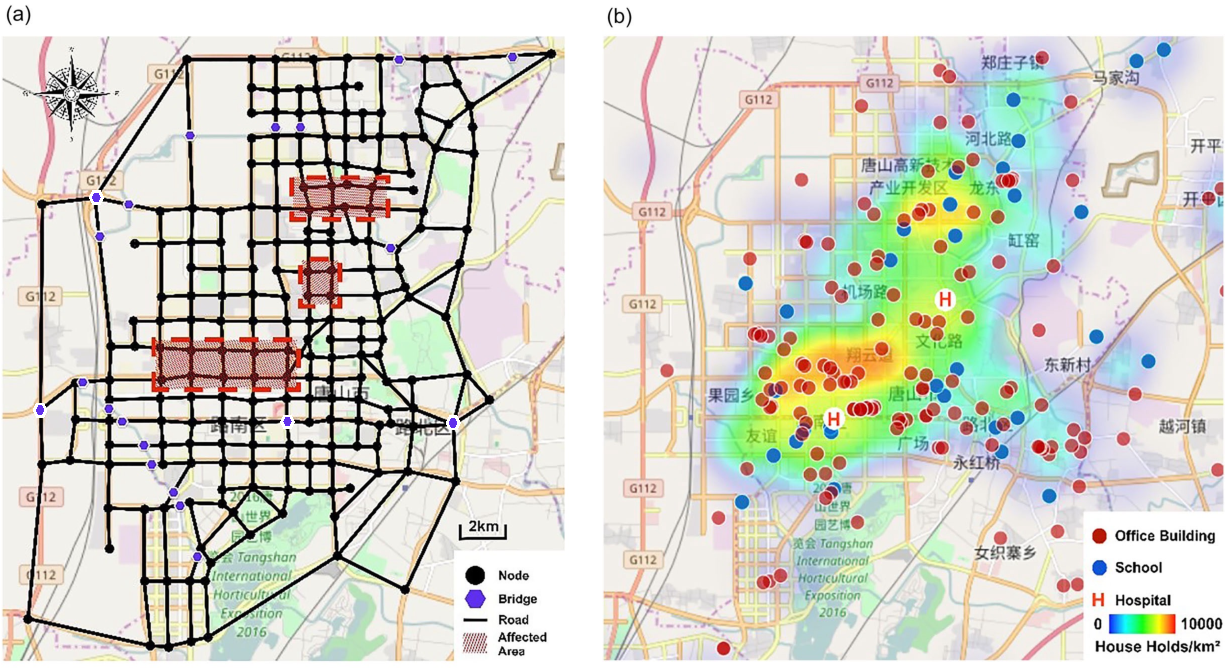
\includegraphics[width=12cm]{fig1.pdf}\\
\caption{Overview of Tangshan City. (a) Transportation network; (b) Population and building locations.}\label{fig1}
\end{figure}

\begin{figure}[!htp]\center
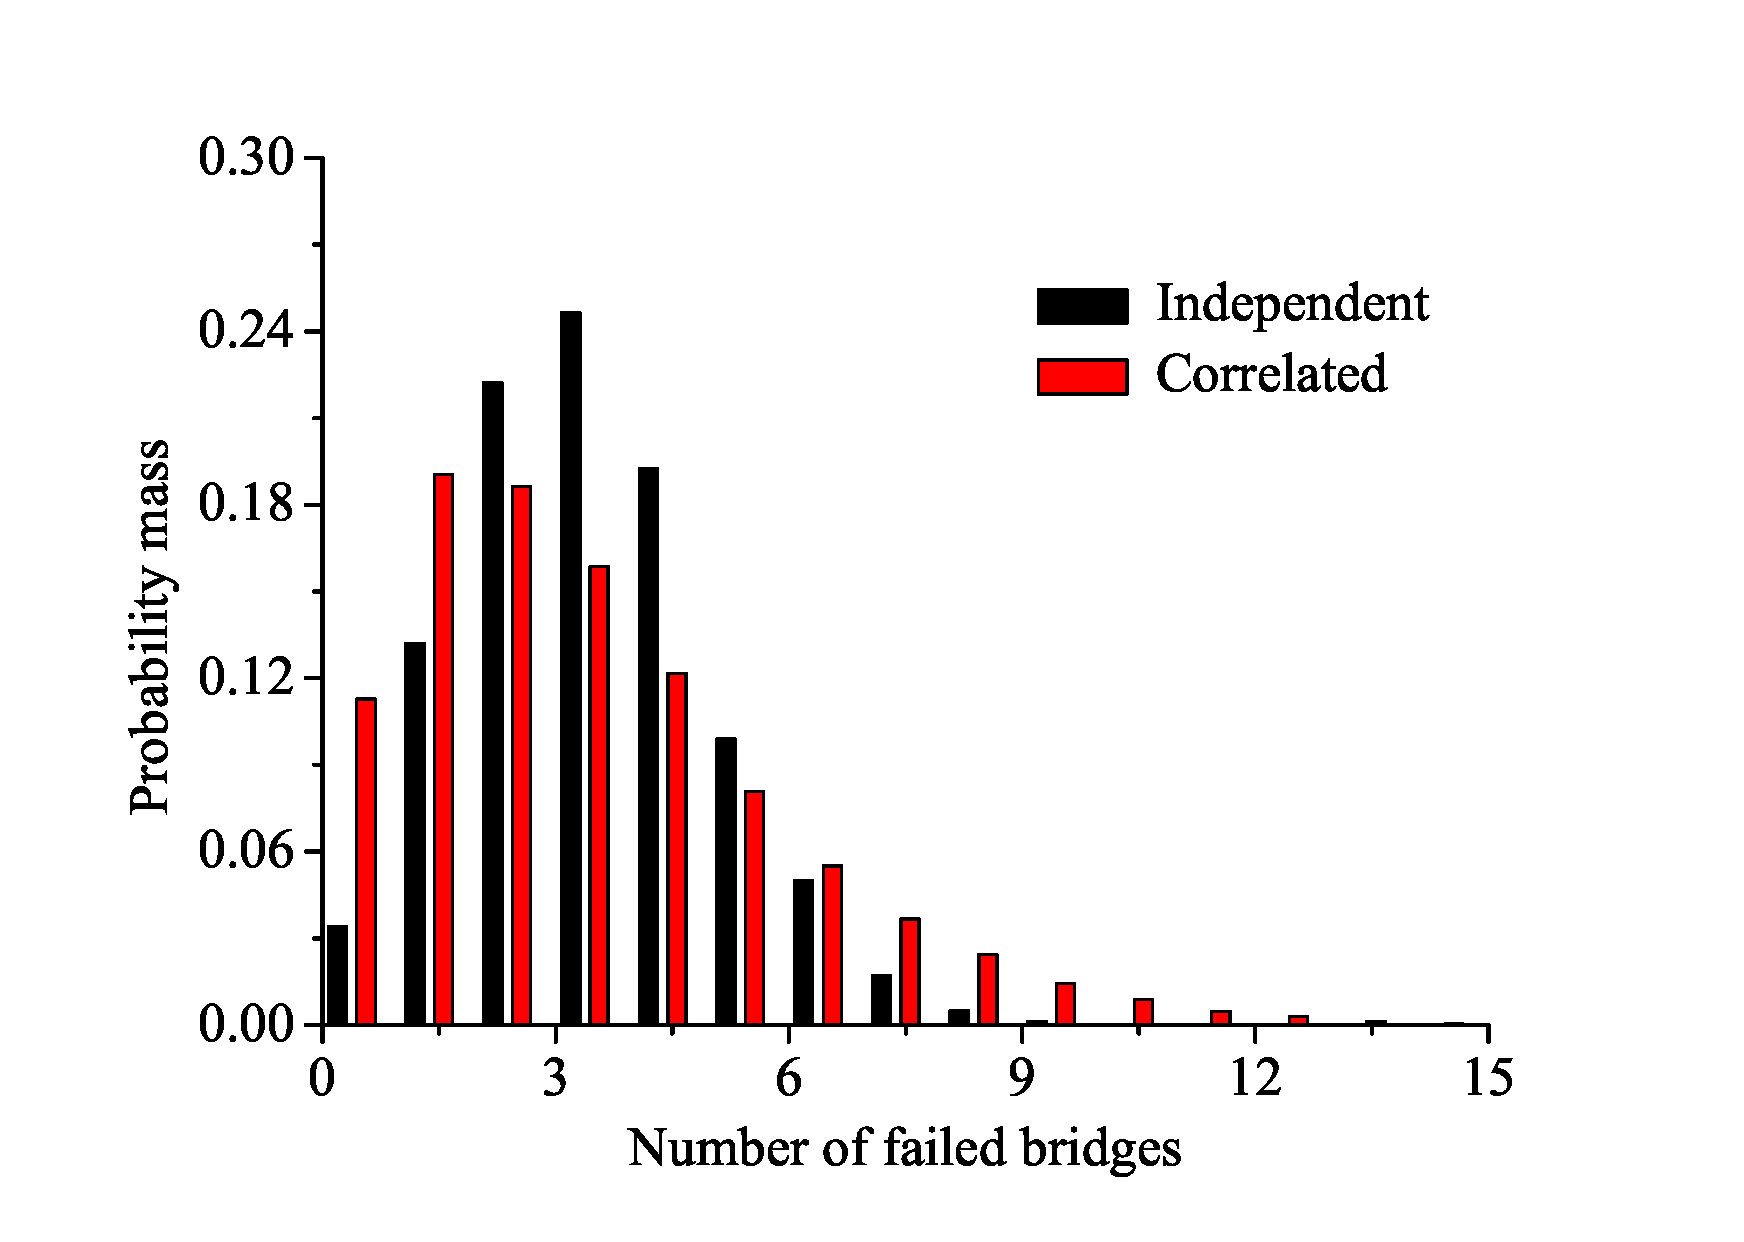
\includegraphics[width=8cm]{fig2.eps}\\
\caption{Probability distribution of the number of failed bridges subjected to an earthquake event.}\label{fig2}
\end{figure}

\subsection{Post-earthquake performance assessment of transportation network}
The post-earthquake performance of Tangshan transportation network is evaluated in this section. First, the gravity model and the user-equilibrium model are used to determine the pre-earthquake traffic congestion, as shown in Figure ~\ref{fig3}. The average travel speed is used to measure the congestion state of each road, which is identified by different colors: red ($<$ 15km/h), orange (15$\sim$25km/h), yellow (25$\sim$35km/h) and green ($>$35km/h). The results in Figure ~\ref{fig3} are validated through the comparison with the 2020 traffic data of Tangshan City. During the morning rush hour, the average speed of all vehicles is 32.5km/h in Figure ~\ref{fig3}, which is consistent with that in the 2020 AutoNavi traffic report (32.34 km/h) \citep{autonavi2020}. Furthermore, the average free-flow traffic speed before earthquake is 47.5 km/h, which is consistent with the recorded 48.5 km/h in \citep{autonavi2020}. Prior to the occurrence of an earthquake, about 23.87\% of the roads are in severe congestion (red), while 64\% are in good condition (green).

\par  In order to estimate the probability profile of the post-earthquake traffic, totally 50,000 simulations are performed. The efficiency of the proposed method can be reflected by the computational time of 20 seconds to simulate one post-earthquake traffic scenario (with a duration of 90 minutes after an earthquake) on an ordinary PC. All the experiments in this section are conducted on a desktop with a configuration of Intel Core i9-9900 K CPU 4.30 GHz ×8,4400 MHz 4 $\times$ 16 GB RAM, 4 TB SSD. For comparison purpose, using an agent-based model as in  \citep{feng2017post}, it would take more than 9 hours to simulate one post-earthquake scenario for the same traffic experiments. Thus, the proposed method can be used to assess the post-hazard performance of a transportation network in a probabilistic and efficient manner. 

\par Following an earthquake event, the distributions of the average vehicle speed of the whole system are estimated for time instants of 10, 30, 60 and 90 minutes after the earthquake, as shown in Figure ~\ref{fig4}. An immediate drop in the average vehicle speed can be observed by comparing Figs.~\ref{fig3} and \ref{fig4}(a). Ten (10) minutes after the earthquake, the average speed decreases from the pre-earthquake 32.5 km/h to 21.7(20.7-22.9)km/h with a standard deviation of 0.8 km/h (here, the two values within the brackets are the characteristic speeds associated with the 10\% and 90\% quantile, respectively). Thirty minutes after the earthquake, the average speed of the system becomes 28.8(25.3-33.6)km/h. While the average speed of the system is increasing, the uncertainty of the system also raised as the standard deviation almost tripled to 3.24 km/h. When it comes to 60 minutes after the earthquake, the average speed of the system further increased to 33.1(28.3-39.9) km/h, and the uncertainty further increases to 4.36 km/h. 

Two peaks are observed in Figure ~\ref{fig4}(c), which represent two modals of the post-earthquake traffic scenario. It is found that these two peaks are dominated by the failure of two independent overpasses. The observation of the two modals demonstrates that the proposed model is capable of capturing the complex post-earthquake traffic behaviors. Ninety minutes after the earthquake, the average speed of the system becomes 37.7(30.2-43.1)km/h, which significantly surpasses the pre-earthquake one, meaning that under most cases the total traffic amount in the transportation system becomes lower than the pre-earthquake level of a typical rush hour. The uncertainty keep going up with a 5.8 km/h standard deviation. The consistency of uncertainty evolution on average vehicle speed reveals that the early stage perturbation of the post-earthquake system might have a prolong impact on the traffic congestion. Therefore, improving management of the post-earthquake traffic would be a cost-efficient strategy to improve the post-earthquake resilience level of a transportation system. It is also observed that the distribution is truncated at a high average speed level. Under some cases, the average vehicle speed reaches 46 km/h, which is close to the free-flow traffic speed (47.5 km/h) of the system. It is hardly possible for the system to reach the free-flow traffic, as reaching free-flow traffic indicates no vehicles on roads. Thus, the system state would be absorbed with the average speed slightly smaller than 47.5 km/h, which leads to the truncation of the distribution.

\par Further, the probabilistic congestion states is obtained 10, 30, 60 and 90 minutes after the earthquake (shown in Figure ~\ref{fig5}). For each percentile (10\%, 50\% and 90\%, the lower quantile representing lower average speed of the system), the average speed is first ranked for all the realizations from the stochastic simulation. Subsequently the scenarios are chosen with the 10\%,50\% and 90\% quantile global average vehicle speeds. Therefore, these probabilistic congestion states are representative of one possible realization of the stochastic simulation. However, as observed in Fig~\ref{fig4}, the system may have some modes. Thus, these quantile plots of the congestion states may fail to cover all the possible spatial distribution of congestion states. Here these plots are employed to represent the typical 10\%,50\% and 90\% congestion states 10, 30, 60 and 90 minutes after the earthquake for quantitative understanding of the simulation results. 

\par It can be observed from Figure ~\ref{fig5} that the heaviest congestion usually occurs at the centre of the city, where the pre-earthquake congestion also likely occurs.  It is also find that, 10 minutes after the earthquake, some suburban/pen-urban areas would also be congested. However, these regions can recover from the congestion faster than the central area of the city. When mapping the scenarios in Figure ~\ref{fig5} with the bridge locations (shown in Figure ~\ref{fig1}), it can be further find that the pen-urban area in southwest corner of Tangshan City, in which a large number of earthquake-prone bridges are located, is also under prolonged traffic congestion under these 10\% quantile cases. Finally, it is with a high likelihood that the system would recover as the pre-earthquake condition in 60 minutes as shown in the 50\% quantile congestion states, which with the 31.7 km/h average vehicle speed is close to pre-earthquake level (32.5 km/h). Under some optimistic cases, e.g. 90\% cases, the transportation system would  approach the free-flow state 90 minutes after the earthquake. However, under some pessimistic cases, there is also a possibility that the congestion remains longer than 90 minutes as shown in the 10\% case with an average speed of 28.4 km/h which is similar to the average speed (28.3 km/h) of the 10\% case 60 minutes after the earthquake.  


\begin{figure}[!htp]\centering
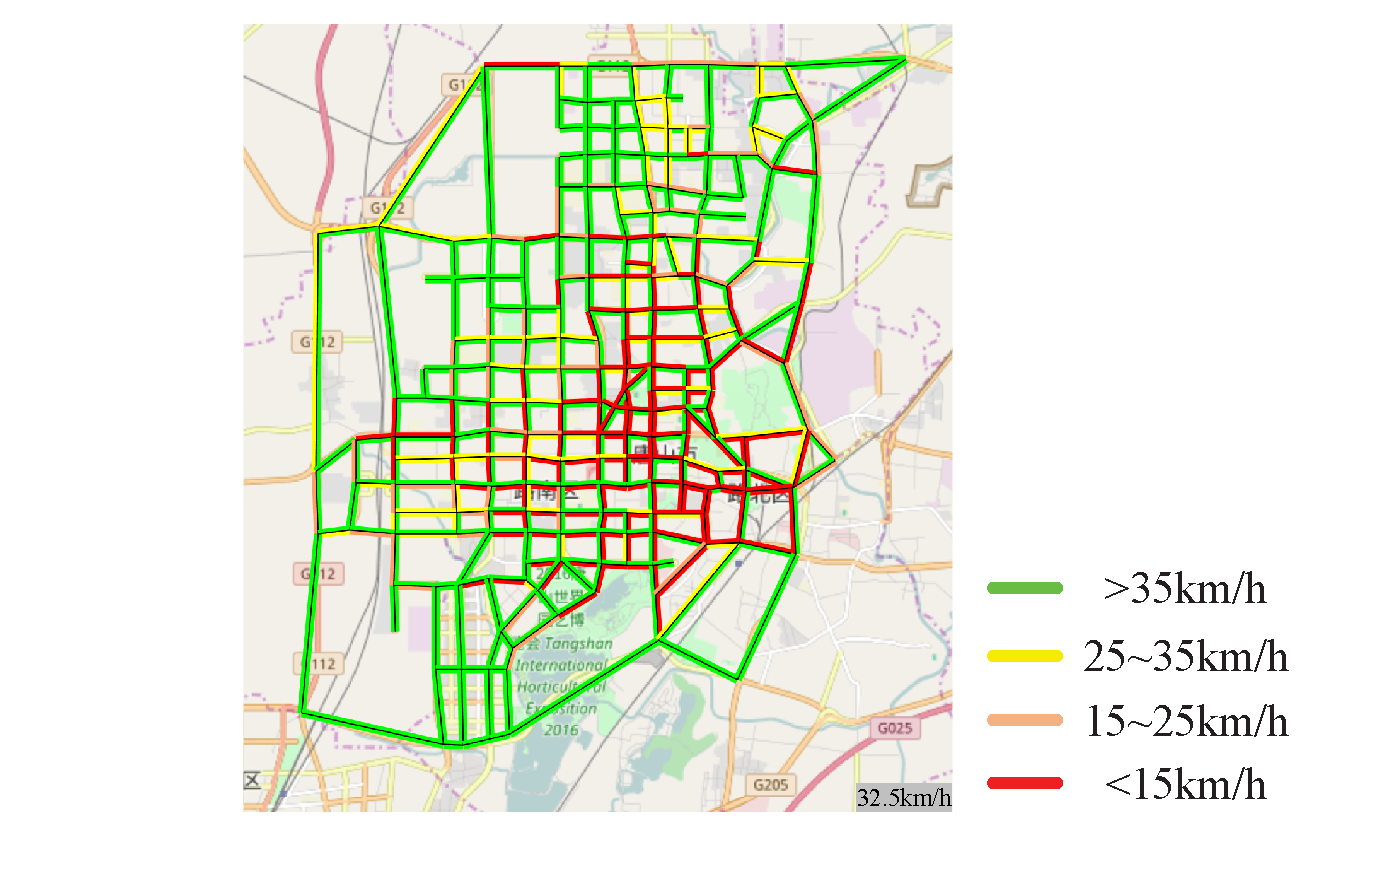
\includegraphics[width=12cm]{fig3.pdf}\\
\caption{\textcolor{black}{Static congestion state before the occurrence of an earthquake}.}\label{fig3}
\end{figure}

\begin{figure}[!htp]\centering
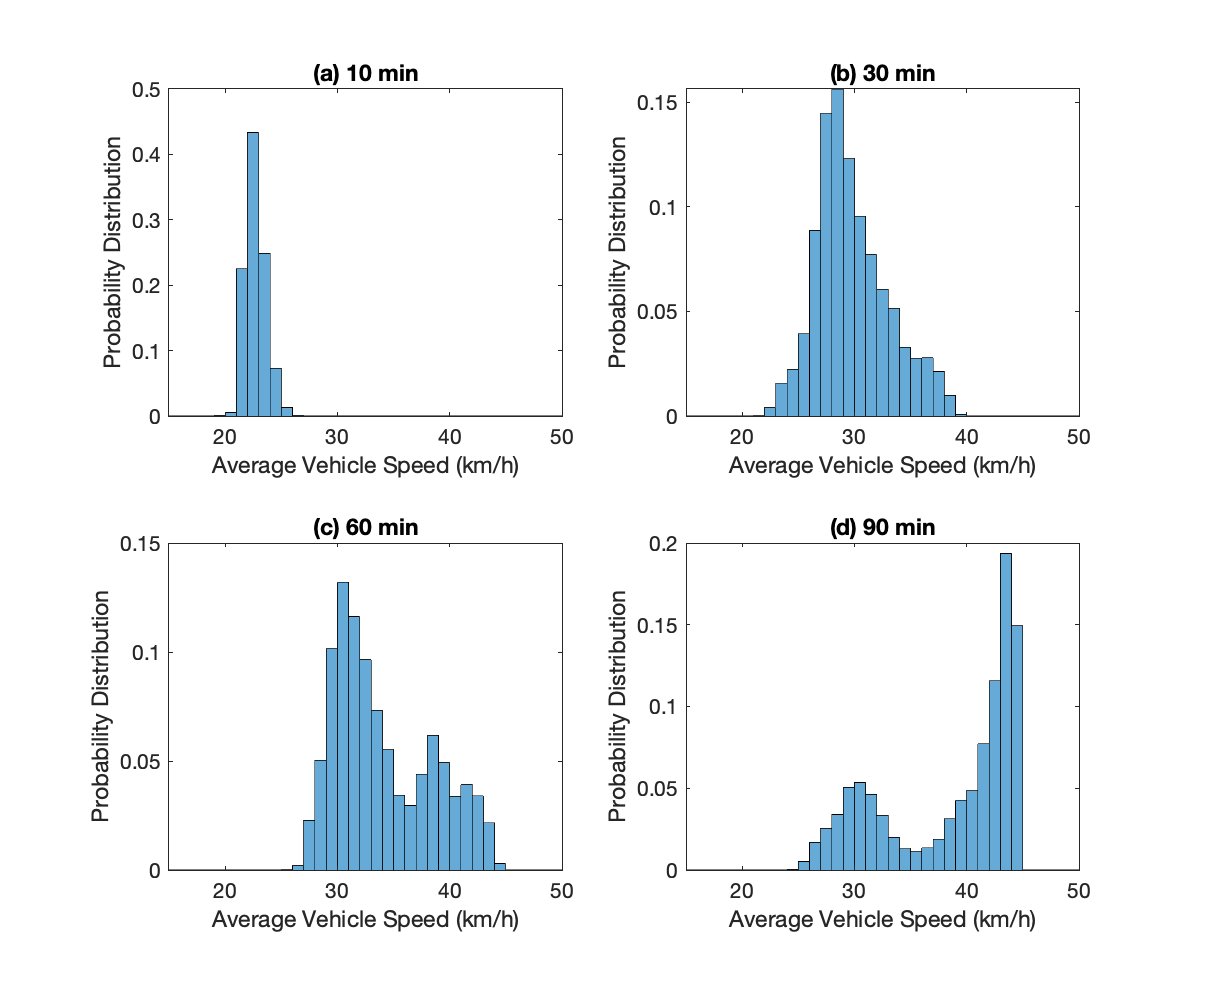
\includegraphics[width=15cm]{fig4.eps}
\caption{\textcolor{black}{The distribution of average speed of the whole traffic system.}}\label{fig4}
\end{figure}

\begin{figure}[!htp]\centering
\includegraphics[width=15cm]{global_traffic1.pdf}\\
\caption{\textcolor{black}{Probabilistic congestion states 10, 30, 60 and 90 minutes after the earthquake. }}\label{fig5}
\end{figure}


\subsection{Evaluation of the transportation network with regard to emergency medical service}
\par The transportation system must remain operational after the earthquake to facilitate the transportation of injured people to hospitals quickly. Thus, the time required for an injured person to receive emergency medical treatment is a suitable index for evaluating the availability of emergency medical services following an earthquake \citep{jones1995emergency,djalali2011facilitators}. 

To illustrate the applicability of the proposed stochastic post-earthquake traffic simulation model, it is also interested in evaluating the post-earthquake emergency transportation level in Tangshan City. Here shows the distribution of traffic time between the two `` AAA '' hospitals (the highest administrative level in China) in Tangshan City in Figure ~\ref{fig6}. This travel time would be important for patient transport under emergency \citep{ceferino2020effective}, e.g. post-earthquake power outage or fire . For each simulation realization, the minimum travel time from one hospital to another is recorded. As a benchmark, the free-flow traffic time between these two hospitals is 9 minutes and the pre-earthquake traffic time between these two hospitals is 14 minutes during the rush hour. It is found that 10 minutes after earthquake, the time cost on average would increase to 18 minutes. 

The travel time cost decrease with a longer duration after the earthquake. Ninety minutes after the earthquake, the time cost on average becomes 12 minutes. Under some optimistic cases, the travel time cost between these two hospitals is close to the free-flow traffic. The uncertainty is larger for the average travel time cost 10 minutes after the earthquake. However, the uncertainty dissipates quickly when it comes to 30/60/90 minutes after earthquake. This observation can be explained by the congestion propagation theory \citep{zhao2016spatio}. The two hospitals (Figure ~\ref{fig1}) are located in the relatively central area of Tangshan City, where the traffic is most congested 10 minutes after the earthquake (Figure ~\ref{fig5}). Thus, the congestion uncertainty level is high in this region with a large vehicle density. The agent level uncertainty accumulates in this region 10 minutes after earthquake. The congestion state of this region 10 minutes after earthquake is dominated by several factors with high uncertainty, e.g. the occurrence of intersection blockage, and the panic rate. At this time (10 minutes after earthquake), most other regions are not congested and the vehicles can always follow the traffic. Thus, the global uncertainty congestion states of the city remains at a lower level. However, the congestion of this central region could propagate among the whole transportation system later on, which increases the global uncertainty level. On the other hand, the congestion state reaches the maximum level 10 minutes after earthquake in this region. As a result, the congestion level could only become lighter in the central region, and the uncertainty of the travel time between these two hospitals dissipates quickly after the earthquake.

\par It is also of interest to obtain the time required for an injured person to receive emergency medical treatment from any of the two hospitals. The network capability in this regard is defined by a delivery time, in terms of hospital delivery area, $A_d$, which is the largest area over which a vehicle can deliver an injured person to the hospital within a specific time. The delivery area depends on the real-time condition of transportation network, but is independent of the density of population in the affected area. That is, available medical services within the delivery area are sufficient to provide necessary services. To determine $A_d$, the shortest time to reach the hospital from each node is calculated and the locations of different links that are within a specified time (e.g., 10 minutes) to the hospital are identified by linear interpolation \citep{feng2017post}.


\par Following the definition in \citep{feng2017post}, the hospital delivery radius $\rho_d$ is calculated as follows, 

\begin{equation}\label{delivery_radius}
\rho_d = \sqrt{A_d/\pi}
\end{equation}

A survey of rescue time in fatal road accidents in the United States in 1990 showed that the rescue time averaged 12 minutes in urban areas and 22 minutes in rural areas \citep{brodsky1990emergency}. Seriously injured persons go into an irremediable state of shock in 15 to 20 minutes. A 10 minutes reduction of the medical response time can be statistically associated with an average decrease of the probability of death by one third, both on motorways and conventional roads \citep{sanchez2010probability}. Thus, suitable metrics are defined for emergency medical services by the 10-min delivery areas (or radii) of the two hospitals in Tangshan City during the morning rush hour before the occurrence of earthquake (considering 5 minutes for stretchering patients into ambulance). Figure \ref{fig7} illustrates this concept; the delivery radii (areas) are 6.0 km and 5.6 km (113 km$^2$ and 98 km$^2$), respectively. 

Following the earthquake, the traffic congestion level becomes more severe immediately, and the 10-min delivery radius suddenly becomes smaller. As the traffic congestion eases, the delivery radius increases gradually. Figs.~\ref{fig8} and \ref{fig9} present the change in the 10-min delivery radius with time after the earthquake for the two hospitals, respectively. Here  solid line is used to represent the 50\% quantile delivery area and dotted lines to represent the 10\% and 90\% quantile delivery areas, respectively. The shade shows the probability distribution of the delivery area. Ten minutes after the earthquake, the delivery radius decreases to 3.8 (1.7-5.5)km in Figure ~\ref{fig8} and 4.8(3.8-6.2)km in Figure ~\ref{fig9}. Thirty minutes after the earthquake, all drivers have regained their composure and the delivery radii increase significantly to 5.2 (3.3-6.2) km and 5.4 (4.2-6.5)km in Figs.~\ref{fig8} and \ref{fig9}. Ninety minutes after the earthquake, the congestion level is eased significantly and the delivery radius is approximately at the pre-earthquake level. This example comprehensively shows the ability of the stochastic traffic model to capture the sophisticated spatial traffic congestion and its evolution over time after an earthquake.   

\begin{figure}[!htp]\centering
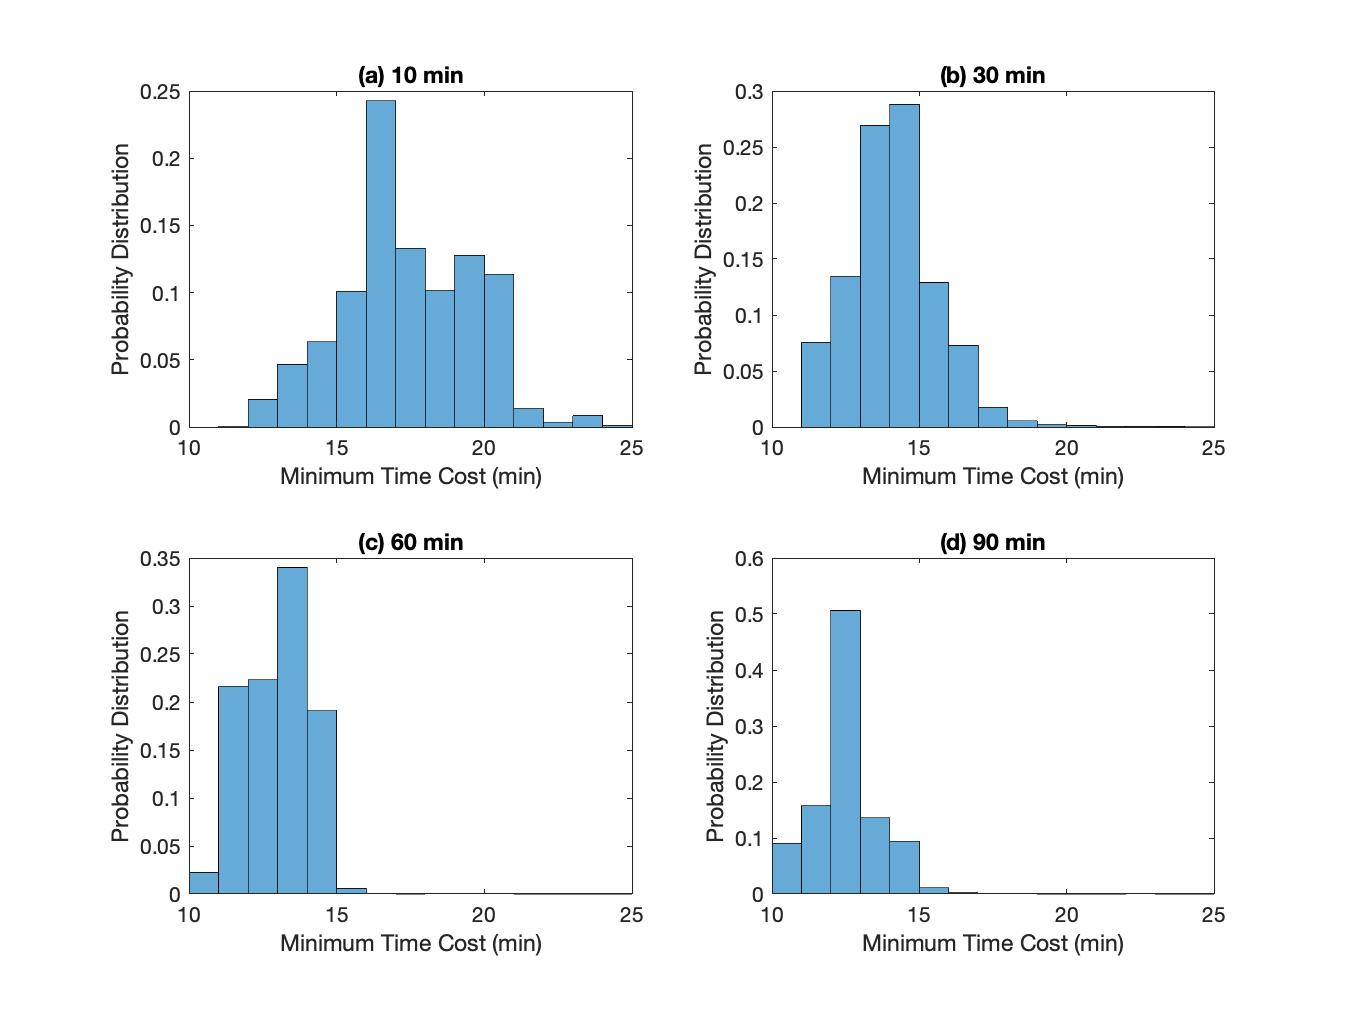
\includegraphics[width = 15cm]{hospital_path.eps}\\
\caption{Distribution of traffic time between two hospitals.}\label{fig6}
\end{figure}

\begin{figure}[!htp]\centering
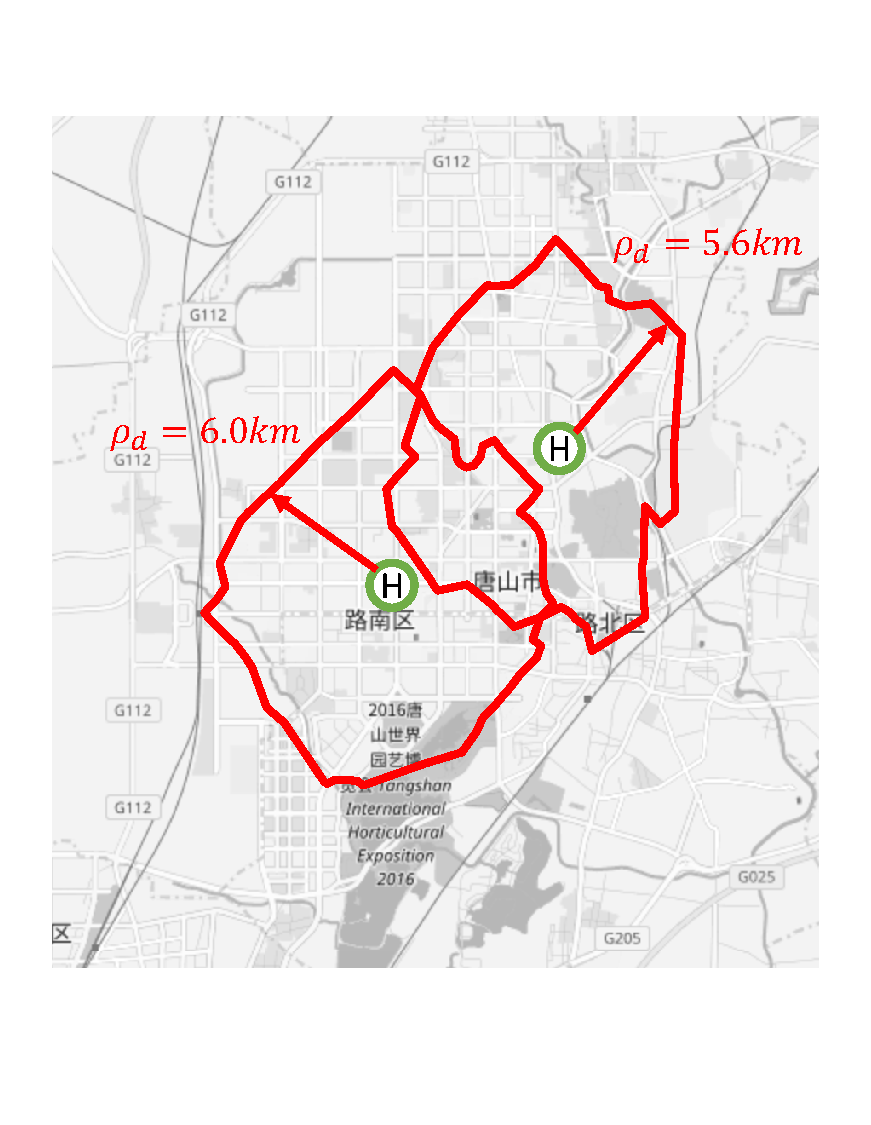
\includegraphics[width=12cm]{initial_contour.pdf}\\
\caption{Pre-earthquake delivery radius of two hospitals.}\label{fig7}
\end{figure}

\begin{figure}[!htp]\centering
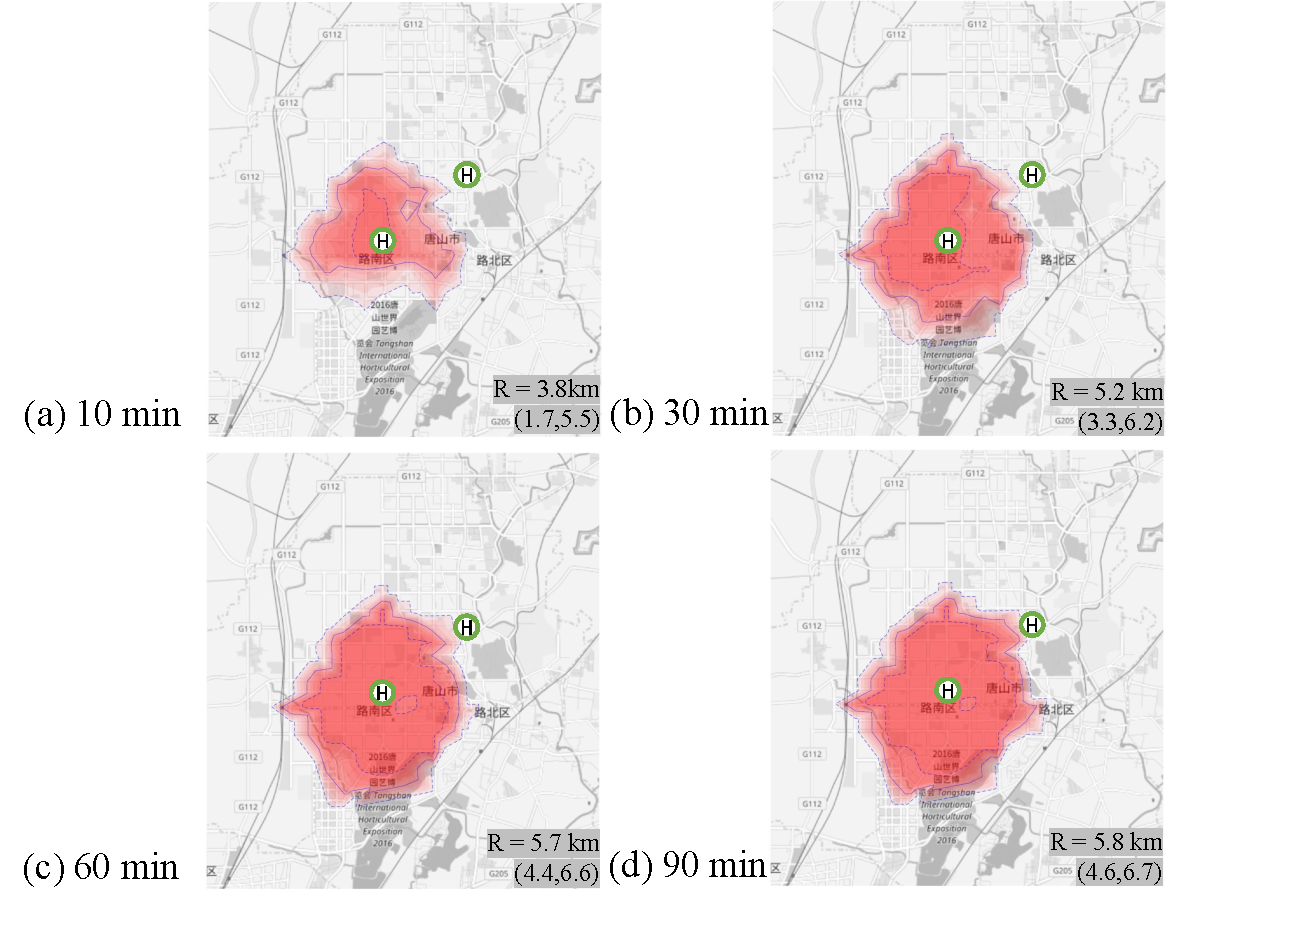
\includegraphics[width=12cm]{contour_hospital_1.pdf}\\
\caption{Post-earthquake delivery area of one hospital.}\label{fig8}
\end{figure}

\begin{figure}[!htp]\centering
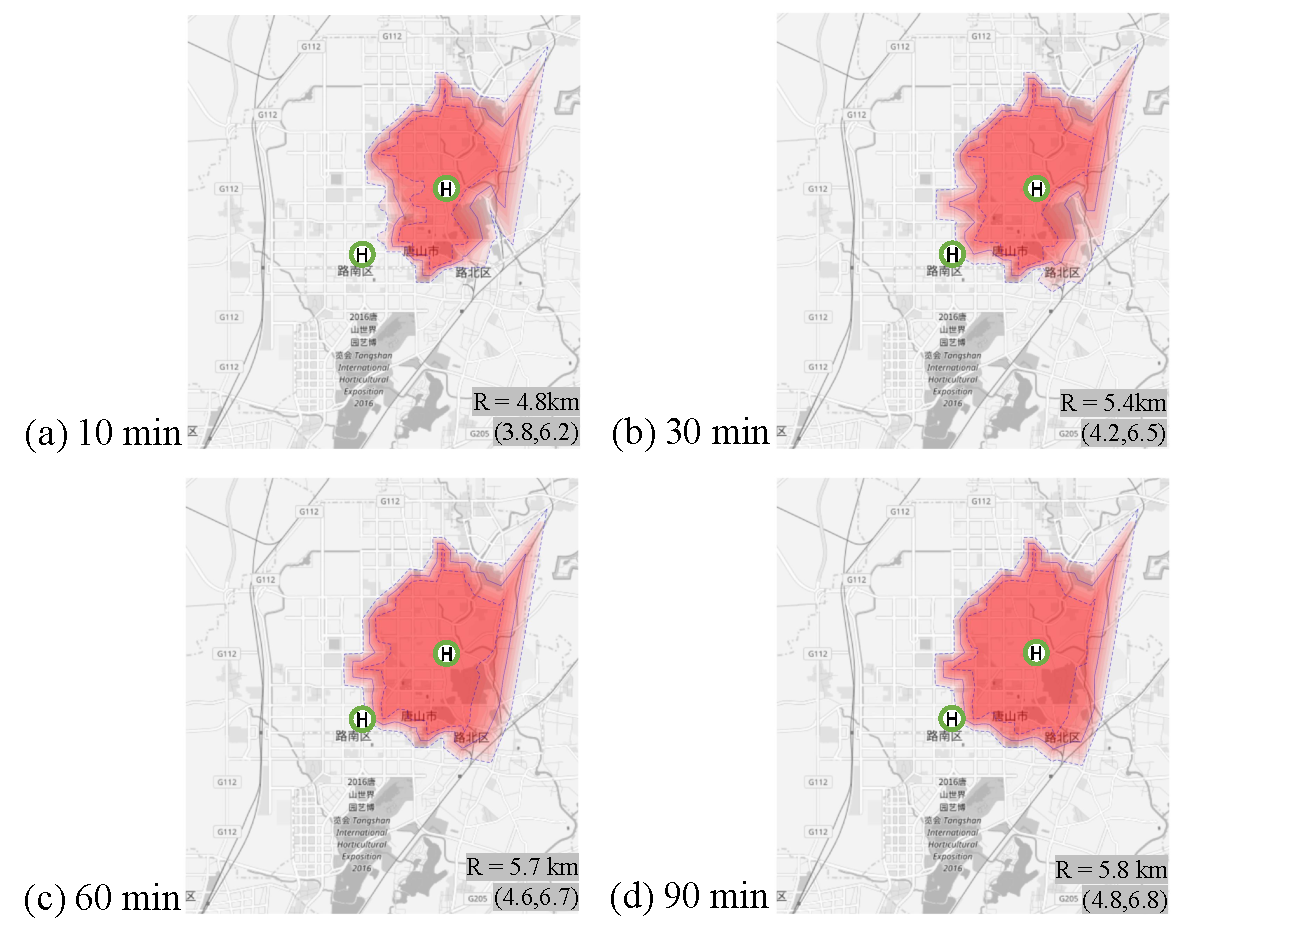
\includegraphics[width=12cm]{contour_hospital_2.pdf}\\
\caption{As of Figure 8 but for another hospital.}\label{fig9}
\end{figure}


\section{Conclusions}

In the context of this research, a novel paradigm is introduced for the estimation of surface transportation systems' performance post-earthquake. The heart of this approach lies in a methodology that facilitates real-time estimates of vehicular spatial distribution across the road network, a critical determinant in the immediate post-earthquake response. These estimations subsequently yield insights into associated travel times and speeds for each road. Furthermore, the proposed methodology inherently encapsulates considerations for the unique characteristics that define post-earthquake traffic dynamics. Factors such as irrationality in driver behavior under the stress of emergency conditions, the immediate change of some drivers' destinations, varying degrees of traffic information accessibility to drivers, and reduced road transport capacity due to infrastructural damage are all accounted for in this comprehensive approach.

The key strength of the proposed approach lies in its ability to facilitate post-earthquake traffic performance estimation in a computationally efficient closed form, thus providing an advantageous alternative to traditional methodologies such as agent-based modelling. This assertion is empirically demonstrated through a case study examining the post-earthquake performance of the Tangshan traffic network, a region with high seismic activity. The assessment parameters encompass multiple aspects, including a Monte Carlo simulation designed to generate probabilistic damage states for both bridges and buildings. This takes into account potential road capacity impediments owing to debris, under the lens of uncertainties associated with seismic hazards.

The results gleaned from the analytical phase underscore the efficacy of the proposed methodology in accurately capturing the modal behavior across spatially distributed traffic scenarios. The road network performance was evaluated, as well as the capacity of emergency medical transport services to convey injured individuals to healthcare facilities. The latter was quantified using the delivery radius of hospitals, evaluated under a probabilistic framework. This significant contribution bolsters our understanding of the response capabilities of transportation systems in seismic events and subsequently informs strategic improvements in disaster management protocols.

\section*{Acknowledgements}
The research described in this paper was supported by the National Key Research and Development Program of China (2016YFC0701404), and the Vice-Chancellor's Postdoctoral Research Fellowship from the University of Wollongong. These supports are gratefully acknowledged.

\printbibliography

\end{document}
